% #######################################
% ########### FILL THESE IN #############
% #######################################
\def\mytitle{Designing XOR Gate using NAND Gates}
\def\mykeywords{}
\def\myauthor{Vemulapalli Bavya Sri}
\def\contact{vemulapallibavya@gmail.com}
\def\mymodule{Future Wireless Communications - IIT Hyderabad (FWC22046)}

% #######################################
% #### YOU DON'T NEED TO TOUCH BELOW ####
% #######################################
\documentclass[10pt, a4paper]{article}
\usepackage[a4paper,outer=1.5cm,inner=1.5cm,top=1.75cm,bottom=1.5cm]{geometry}
\twocolumn
\usepackage{graphicx}
\graphicspath{{./images/}}
%colour our links, remove weird boxes
\usepackage[colorlinks,linkcolor={black},citecolor={blue!80!black},urlcolor={blue!80!black}]{hyperref}
%Stop indentation on new paragraphs
\usepackage[parfill]{parskip}
%% Arial-like font
\usepackage{lmodern}
\renewcommand*\familydefault{\sfdefault}
%Napier logo top right
\usepackage{watermark}
%Lorem Ipusm dolor please don't leave any in you final report ;)
\usepackage{lipsum}
\usepackage{xcolor}
\usepackage{listings}
%give us the Capital H that we all know and love
\usepackage{float}
%tone down the line spacing after section titles
\usepackage{titlesec}
%Cool maths printing
\usepackage{amsmath}
%PseudoCode
\usepackage{algorithm2e}

\titlespacing{\subsection}{0pt}{\parskip}{-3pt}
\titlespacing{\subsubsection}{0pt}{\parskip}{-\parskip}
\titlespacing{\paragraph}{0pt}{\parskip}{\parskip}
\newcommand{\figuremacro}[5]{
    \begin{figure}[#1]
        \centering
        \includegraphics[width=#5\columnwidth]{#2}
        \caption[#3]{\textbf{#3}#4}
        \label{fig:#2}
    \end{figure}
}

\lstset{
  escapeinside={/@}{@/}, language=C++,
  basicstyle=\fontsize{8.5}{12}\selectfont,
  numbers=left,numbersep=2pt,xleftmargin=2pt,frame=tb,
    columns=fullflexible,showstringspaces=false,tabsize=4,
    keepspaces=true,showtabs=false,showspaces=false,
    backgroundcolor=\color{white}, morekeywords={inline,public,
    class,private,protected,struct},captionpos=t,lineskip=-0.4em,
  aboveskip=10pt, extendedchars=true, breaklines=true,
  prebreak = \raisebox{0ex}[0ex][0ex]{\ensuremath{\hookleftarrow}},
  keywordstyle=\color[rgb]{0,0,1},
  commentstyle=\color[rgb]{0.133,0.545,0.133},
  stringstyle=\color[rgb]{0.627,0.126,0.941}
}

\thiswatermark{\centering \put(0,-90.0){
\includegraphics[scale=0.05]{iith.jpg}} }
\title{\mytitle}
\author{\myauthor\hspace{1em}\\\contact\\\hspace{0.5em}\hspace{0.5em}\mymodule}
\date{}
\hypersetup{pdfauthor=\myauthor,pdftitle=\mytitle,pdfkeywords=\mykeywords}
\sloppy
% #######################################
% ########### START FROM HERE ###########
% #######################################
\begin{document}
  \maketitle
\tableofcontents

\begin{abstract}
    This manual shows how to design 2-input XOR gate using 4 NAND gates.
\end{abstract}

\section{Introduction}
\subsection{XOR Gate}

   The full form of XOR gate is Exclusive-OR gate. Its function is the same as that of OR gate but with few output changes. The output of an Exclusive-OR gate goes “HIGH” when its two input terminals are at “DIFFERENT” logic levels with respect to each other. In other case the output goes "LOW".
        
         Boolean Expression Q = A.B' + A'.B 
\begin{figure}[H]
    \centering
    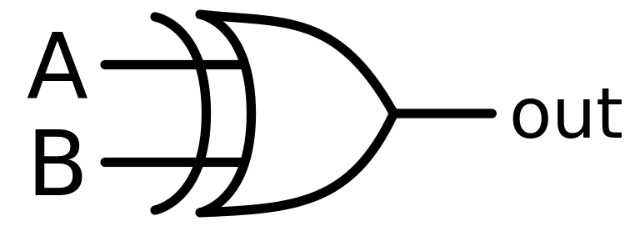
\includegraphics[scale=0.5]{XOR Gate.png}
    \caption{XOR Gate}
    \label{fig:XOR}
\end{figure}

\subsection{XOR Gate using NAND Gates}

XOR gate is achieved by combining standard logic gates together to form more complex gate functions that are used extensively in building arithmetic logic circuits, computational logic comparators and error detection circuits. One can construct a XOR gate by using minimum of 4 NAND gates. It is also possible to design an XOR gate using more than four NAND gates. 


\begin{figure}[H]
    \centering
    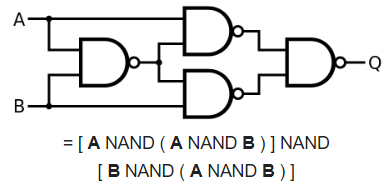
\includegraphics{XOR using NAND.png}
    \caption{XOR gate with 4 NAND gates}
    \label{fig XOR NAND}
\end{figure}


\section{Truth Table}

\begin{table}[H]
 \begin{center}
    \begin{tabular}{|l|c|c|c|c|c|c|c|c} \hline \textbf{A}
  & \textbf{B} & \textbf{Q} \\
 \hline
0&0&0 \\ \hline
0&1&1 \\ \hline
1&0&1\\ \hline
1&1&0  \\ \hline
\end{tabular}   
\end{center}
\caption{Truth table}
\label{table 1}
\end{table}


\section{Components}



\begin{table}[H]
 \begin{center}
    \begin{tabular}{|l|c|c|c|c|c|c} \hline \textbf{Component}
  & \textbf{Value} & \textbf{Quantity} \\
 \hline
Resistor & 220 ohm & 1 \\ \hline
Arduino & UNO & 1 \\ \hline
Bread board &  & 1 \\ \hline
Jumper wires & M-M & 4\\ \hline
\end{tabular}   
\end{center}
\caption{Components}
\label{table 2}
\end{table}



\section{Hardware}

Make connections between LED and Arduino as shown in Table 3.

\begin{table}[H]
 \begin{center}
    \begin{tabular}{|l|c|c|c|c|c|c|c|c} \hline\textbf{Arduino} & \textbf{13} & \textbf{GND} \\ \hline
 \textbf{Led} & \textbf{+VE} & \textbf{-VE}\\ \hline
\end{tabular}   
\end{center}
\caption{Connections}
\label{table 3}
\end{table}


\section{Software}

Execute the following program after downloading it.

\begin{table}[H]
 \begin{center}
    \begin{tabular}{|l|c|c|c|c|c|c|c|c}\hline\textbf{https://raw.githubusercontent.com}\\
    \textbf{BavyaVemulapalli/FWC-IITH/main/AvrGcc/Codes/avr.c} \\ \hline
\end{tabular}   
\end{center}
\end{table}


\section{Conclusion}
We observe the LED going LOW and HIGH depending on the operation of 2-input XOR gate using NAND gates.



\end{document}